\chapter[Data analysis]{Data analysis}

\section[Offline selection of the events]{Offline selection of the events}

In order to perform the data analysis, a full analysis framework have been developed using MATLAB. The selection of the interesting events will be described chronologically, as it's performed in the analysis program.

\subsection[Data collected from the PXI]{Data collected from the PXI}

As mentioned in the previous chapter, the data acquisition is performed from a real-time LabVIEW program running into the PXI crate. When an event hits at least one of the online triggers is saved into the crate's disk. Every 8 hours, the crate assemble a data file and stores it in TDMS format \cite{NI:TDMS}. To proceed with the analysis, the files are merged joining all the data of the same day together in a new data file. The original data are anyway kept stored. All these actions were found already implemented in the system at the beginning of this work.

The kind of events that are collected by the PXI crate have two natures:
\begin{enumerate}
\item Interlock pulses: an event that triggered one of the online interlock. If available, the two precedent pulses are saved.
\item Backup pulses: if no event triggers an online interlock, a pulse every minute is saved.
\end{enumerate}
The first ones are sent to the next analysis step, the second ones are analysed separately to check the running condition of the accelerator and the RF systems.


\subsection[Power spikes detection]{Power spikes detection}

A key operational issue is the presence of power spikes, that sometimes are detected in the systems. The main characteristics of these events are:
\begin{itemize}
\item Short duration: normally in the range 10-100 ns
\item Very high power burst: it can reach 60-70 MW or even more 
\end{itemize}
The fist point makes the spikes easily detectable using a frequency filter to detect signals of that short duration. 

 After careful investigation, the origin of the spikes has been addressed to the TWT. It has to be pointed out that the frequency of the spikes is anyway low compared to the rate of the breakdown, and that after the first runs the replacement of a very active tube improved a lot the performance. As can be seen in Fig. \ref{spikesAndDetuning}, the spike can happen everywhere in the pulse.

 \begin{figure}[h]
 \centering
   \subfigure[Power spike in the prepulse]
   {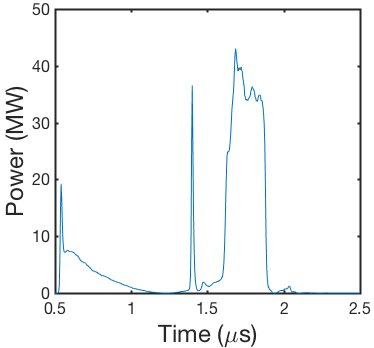
\includegraphics[scale=0.48]{pictures/spike1.png}}
 \hspace{2mm}
 \subfigure[Power spike in the compressed pulse]
   {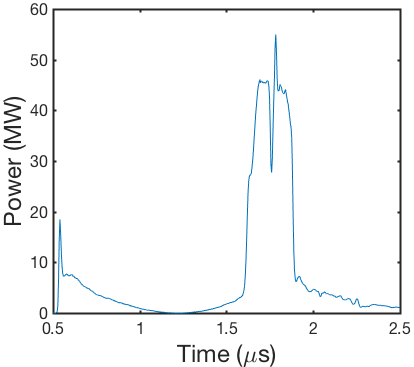
\includegraphics[scale=0.46]{pictures/spike2.png}}
 \caption{Cavity input power signal for two different spikes. Spikes can happen anywhere in the signal, even if the experience suggest that are more likely in the compressed pulse.}
 \label{spikesAndDetuning}
 \end{figure}


When a spike gets detected, the correspondent interlock is sorted out, and also the followings for a given period of time (generally 90 s). The reason is that it is believed that the burst of power brought from the spike may trigger strong breakdowns that damage the surface. This creates new emitters that triggers new breakdowns as soon as the system don't reach an equilibrium. The waiting time before restarting to count the breakdowns gives time to the surface to cool down and get reconditioned.


\subsection[Pulse compressor tuning issues]{Pulse compressor tuning issues}

RF tests of accelerating cavities are carried out using the CLIC nominal pulse shown in Fig. \ref{detuning_fig} (a). This comes from the necessity to find a common test protocol for accelerating cavities, that has also to match the different pulse length of the RF foreseen in the three stages of the CLIC implementation. To meet these requirements, the CLIC nominal pulse is made of a filling (or rising) time of 70 ns and a flat-top 180 ns long.

A common operational issue is the detuning of the pulse compressor, that provokes an imperfect shape of the RF pulse. This event does not constitute an issue for the implementation of CLIC (unless implemented in the klystron option). Anyway excessively detuned running periods are sorted out, hence far from the wanted experimental conditions. 

The origin of the detuning is the difference of the total volume of the pulse compressor's cavities. This is controlled changing the cooling water temperature, but as any other thermal system needs time for the regulation \cite{Woolley:CWS2016}. The detuning is a particular issue in summer, when the thermal excursion during the day is particularly high.

As general rule a slight detuning of the pulse is tolerated, and it is not possible to get rid of it because the regulation of the temperature of the chillers act dynamically and needs time to compensate the variations. On the other hand the data are not considered in case of extreme detuning such as in Fig. \ref{detuning_fig} (b) and (c), where the box-shape of the pulse is not recognisable anymore. 

 \begin{figure}
 \centering
  \subfigure[CLIC nominal pulse]
   {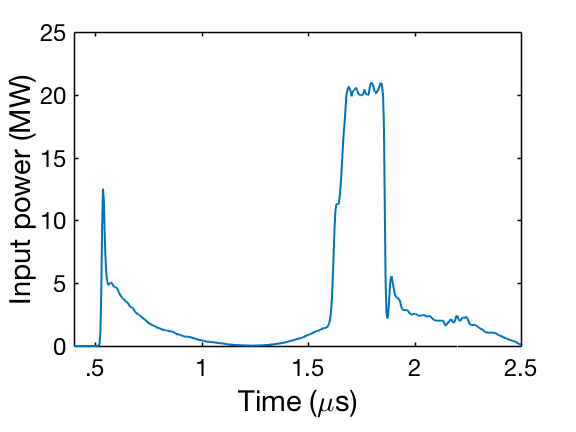
\includegraphics[scale=0.45]{pictures/CLIC_nominal_pulse.png}}
  \subfigure[Pulse compressor undertuned]
   {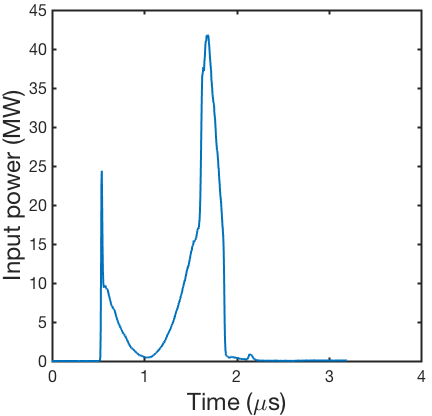
\includegraphics[scale=0.42]{pictures/Undertuning.png}}
 \hspace{2mm}
 \subfigure[Pulse compressor overtuned]
   {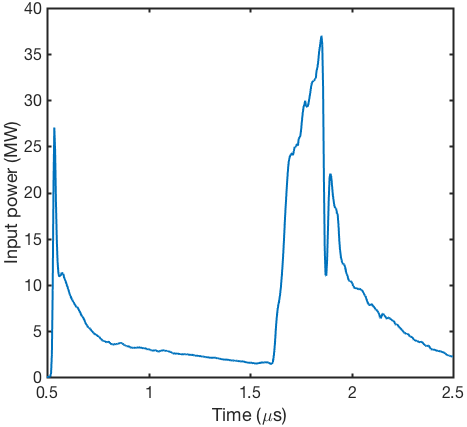
\includegraphics[scale=0.41]{pictures/Overtuning.png}}
\caption{The CLIC nominal pulse and two extreme cases of detuning of the pulse compressor.}
 \label{detuning_fig}
 \end{figure}


\subsection[The metric]{The metric}

The key issue in the analysis of the vacuum arcs in the accelerating cavity is to understand if the breakdown happened in the accelerating cavity, and sort out the breakdowns happening elsewhere. For this purpose two quantities are evaluated:
\begin{equation}
\frac{ E_{INC} -  E_{REF}   }{  E_{INC} +  E_{REF}   }
\end{equation}
\begin{equation}
\frac{ E_{INC} -  E_{TRA}   }{  E_{INC} +  E_{TRA}   }
\end{equation}
by doing so two distinct regions gets highlighted (see Fig. \ref{Metric_plot}). The upper left region is made of the fake interlocks and the breakdown that happen upstream the structure under test. The events happening in the structure end up in the lower right area on the plot.

\begin{figure}[h]
\centering 
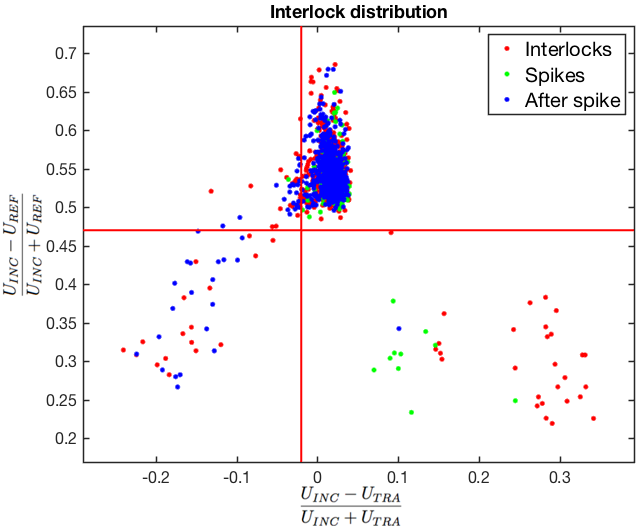
\includegraphics[scale=0.6]{pictures/metric_plt.png}
\caption{Metric plot for an unloaded run. Data grouped in two different regions are clearly visible. The lowest region is containing the interesting interlocks, that are sent to the next analysis step}
\label{Metric_plot}
\end{figure}


The selection based on the metric would be already sufficient to produce good results, with no need of further refining.



\subsection[Additional criteria for runs with beam]{Additional criteria for runs with beam}

During the experiments with beam, two additional conditions have to be met to consider an interlock as a breakdown in the accelerating structure
\begin{enumerate}
\item The beam has to be present during the pulse
\item In the case of a breakdown happened during a period without beam, the 
\end{enumerate}











\section[Time and space positioning of the breakdowns]{Time and space positioning of the breakdowns}







\section[Beam induced RF]{Beam induced RF}
